\documentclass[aspectratio=169]{beamer}\usepackage[]{graphicx}\usepackage[]{xcolor}
% maxwidth is the original width if it is less than linewidth
% otherwise use linewidth (to make sure the graphics do not exceed the margin)
\makeatletter
\def\maxwidth{ %
  \ifdim\Gin@nat@width>\linewidth
    \linewidth
  \else
    \Gin@nat@width
  \fi
}
\makeatother

\definecolor{fgcolor}{rgb}{0.345, 0.345, 0.345}
\newcommand{\hlnum}[1]{\textcolor[rgb]{0.686,0.059,0.569}{#1}}%
\newcommand{\hlsng}[1]{\textcolor[rgb]{0.192,0.494,0.8}{#1}}%
\newcommand{\hlcom}[1]{\textcolor[rgb]{0.678,0.584,0.686}{\textit{#1}}}%
\newcommand{\hlopt}[1]{\textcolor[rgb]{0,0,0}{#1}}%
\newcommand{\hldef}[1]{\textcolor[rgb]{0.345,0.345,0.345}{#1}}%
\newcommand{\hlkwa}[1]{\textcolor[rgb]{0.161,0.373,0.58}{\textbf{#1}}}%
\newcommand{\hlkwb}[1]{\textcolor[rgb]{0.69,0.353,0.396}{#1}}%
\newcommand{\hlkwc}[1]{\textcolor[rgb]{0.333,0.667,0.333}{#1}}%
\newcommand{\hlkwd}[1]{\textcolor[rgb]{0.737,0.353,0.396}{\textbf{#1}}}%
\let\hlipl\hlkwb

\usepackage{framed}
\makeatletter
\newenvironment{kframe}{%
 \def\at@end@of@kframe{}%
 \ifinner\ifhmode%
  \def\at@end@of@kframe{\end{minipage}}%
  \begin{minipage}{\columnwidth}%
 \fi\fi%
 \def\FrameCommand##1{\hskip\@totalleftmargin \hskip-\fboxsep
 \colorbox{shadecolor}{##1}\hskip-\fboxsep
     % There is no \\@totalrightmargin, so:
     \hskip-\linewidth \hskip-\@totalleftmargin \hskip\columnwidth}%
 \MakeFramed {\advance\hsize-\width
   \@totalleftmargin\z@ \linewidth\hsize
   \@setminipage}}%
 {\par\unskip\endMakeFramed%
 \at@end@of@kframe}
\makeatother

\definecolor{shadecolor}{rgb}{.97, .97, .97}
\definecolor{messagecolor}{rgb}{0, 0, 0}
\definecolor{warningcolor}{rgb}{1, 0, 1}
\definecolor{errorcolor}{rgb}{1, 0, 0}
\newenvironment{knitrout}{}{} % an empty environment to be redefined in TeX

\usepackage{alltt}
\usetheme{gotham}

% \setbeamercolor{block~title}{
%   
% }

	\usepackage{standalone}
	\usepackage{tikz}
	\usepackage{pgfplots}
	\usepackage{tabularray} % Typeset tabulars and arrays (contains equivalent of longtable, booktabs and dcolumn at least)
		\UseTblrLibrary{booktabs} % to load extra commands from booktabs
	\usepackage{changepage}
	\usepackage{minted}
		\definecolor{codeback}{rgb}{0.90,0.91,0.92}
		\definecolor{codebackdark}{rgb}{0.10,0.11,0.12}

	\newcommand{\famName}[1]{\textsc{#1}}
	\newcommand{\themename}{\textbf{\textsc{Gotham}}}
\IfFileExists{upquote.sty}{\usepackage{upquote}}{}
\begin{document}

\section{Introduction}

\begin{frame}{Synonyms and Definitions}

There are several terms that have been used as synonyms with state space models (SSMs):

\begin{itemize}
  \item Mechanistic model
  \item Hidden Markov model (HMM)
  \item Partially observed Markov process (POMP) model
\end{itemize}

I will begin by defining how these terms are used in my thesis.

\end{frame}

\begin{frame}{State Space Models (SSM)}
  I follow the definition used by \citet{durbin12} for a SSM.
  
  \begin{itemize}
  \item $\bm{Y}_{1}, \bm{Y}_2, \ldots, \bm{Y}_{N}$ are observed time series. 
  Observations occur at time points $t_1, \ldots, t_N$, and can be vector valued. 
  \item A SSM introduces unobservable (latent) states $\bm{X}_1, \ldots, \bm{X}_N$ at the same observation times.
  These latent variables are connected to the observations, in a way defined by the model.
  \item We often include an initial value for the latent states, $\bm{X}_0$.
  \end{itemize}
  
  I will adopt the shorthand $t_{\seq{1}{N}} = (t_1, \ldots, t_N)$, $\bm{Y}_{\seq{1}{N}} = (\bm{Y}_{1}, \ldots, \bm{Y}_{N})$, and $\bm{X}_{\seq{0}{N}} = (\bm{X}_0, \ldots, \bm{X}_N)$.

\end{frame}

\begin{frame}{Likelihood function}

  We assume that the random variables $\bm{Y}_{\seq{1}{N}}$, $\bm{X}_{\seq{0}{N}}$ have a joint probability density $f_{\bm{X}_{\seq{0}{N}}, \bm{Y}_{\seq{1}{N}}}(\bm{x}_{\seq{0}{N}}, \bm{y}_{\seq{1}{N}}; \, \paramVec)$ with respect to some dominating measure (Lebesgue or counting).
  
  $\paramVec$ is a parameter vector $\paramVec \in \R^{d_\paramVec}$ that indexes the model (unknown).
  
  Because only $\bm{Y}_{\seq{1}{N}}$ is observable, the likelihood function involves a high-dimensional integral: 
  
\begin{eqnarray}
  \label{eq:likedef}
  \mathcal{L}(\paramVec; \bm{y}^*) = f_{\bm{Y}_{1:N}}\big(\bm{y}_{1:N}^*; \, \paramVec\big) = \int f_{\bm{X}_{\seq{0}{N}}, \bm{Y}_{\seq{1}{N}}}\big(\bm{x}_{\seq{0}{N}}, \bm{y}_{\seq{1}{N}}^*;\, \paramVec\big) \, d\bm{x}_{\seq{0}{N}}.
\end{eqnarray}

\end{frame}

\begin{frame}{POMP models}

A common approach is to treat SSMs as partially observed Markov process (POMP) models. We make the following assumptions: 
\begin{itemize}
  \item We assume that the latent variables are a Markov process
  $$
  f_{\bm{X}_{n} | \bm{X}_{1:n-1}}(\bm{x}_{n} | \bm{x}_{1:n-1}; \, \paramVec) = f_{\bm{X}_{n} | \bm{X}_{n-1}}(\bm{x}_{n} | \bm{x}_{n-1}; \, \paramVec).
  $$
  \item Measurements are conditionally independent
  $$
  f_{\bm{Y}_{n} | \bm{X}_{1:N}, \bm{Y}_{-n}}(\bm{y}_{n} | \bm{x}_{0:N}, \bm{y}_{-n}; \, \paramVec) = f_{\bm{Y}_{n} | \bm{X}_{n}}(\bm{y}_{n} | \bm{x}_{n}; \, \paramVec).
  $$
\end{itemize}
With these assumptions, we can express the joint density as
\begin{eqnarray}
\label{eq:jointLik}
f_{\bm{X}_{0:N}, \bm{Y}_{1:N}}\big(\bm{x}_{0:N}, \bm{y}_{1:N};\, \paramVec\big) = f_{\bm{X}_0}\big(\bm{x}_0;\, \paramVec\big)\prod_{n = 1}^N f_{\bm{X}_n|\bm{X}_{n-1}}\big(\bm{x}_{n}|\bm{x}_{n-1}; \, \paramVec\big)f_{\bm{Y}_n|\bm{X}_{n}}\big(\bm{y}_n|\bm{x}_{n}; \, \paramVec\big).
\end{eqnarray}
\end{frame}

\begin{frame}{POMP pieces}
  $$
  f_{\bm{X}_0}\big(\bm{x}_0;\, \paramVec\big)\prod_{n = 1}^N f_{\bm{X}_n|\bm{X}_{n-1}}\big(\bm{x}_{n}|\bm{x}_{n-1}; \, \paramVec\big)f_{\bm{Y}_n|\bm{X}_{n}}\big(\bm{y}_n|\bm{x}_{n}; \, \paramVec\big)
  $$
  \begin{itemize}
    \item The initialize density (or initializer): $f_{\bm{X}_0}\big(\bm{x}_0;\, \paramVec\big)$.
    \item The transition density (or process model): $f_{\bm{X}_n|\bm{X}_{n-1}}\big(\bm{x}_{n}|\bm{x}_{n-1}; \, \paramVec\big)$. 
    \item The measurement density (or model): $f_{\bm{Y}_n|\bm{X}_{n}}\big(\bm{y}_n|\bm{x}_{n}; \, \paramVec\big)$.
  \end{itemize}
  The latent states can be defined as a continuous time process with values in-between measurement times. 
\end{frame}

\begin{frame}
\begin{figure}[!ht]
\begin{knitrout}
\definecolor{shadecolor}{rgb}{0.969, 0.969, 0.969}\color{fgcolor}
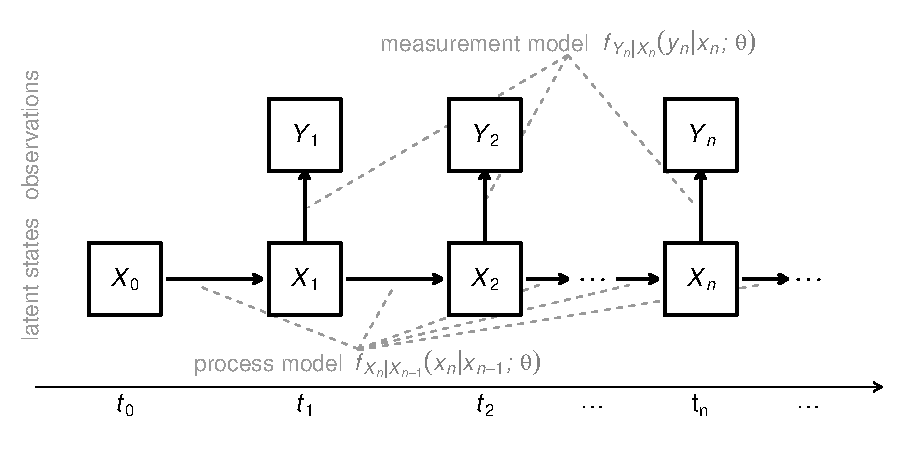
\includegraphics[width=0.75\maxwidth]{figure/pompDiagram-1} 
\end{knitrout}
\caption{\label{fig:pompDiagram}A flow diagram representing an arbitrary POMP model. Modified figure from SBIED course (King, Ionides).}
\end{figure}

Each of the SSMs considered in this thesis are POMP models.

\end{frame}

\begin{frame}{Other synonyms and definitions}
  Other common terms that are sometimes used as synonyms are used for special cases 
  \begin{block}{Mechanistic Model}
    A SSM (or POMP) where the evolution of latent variables is dictated by equations that mimic real-world mechanisms. 
  \end{block}
  
  \begin{block}{Hidden Markov Model (HMM)}
    A SSM (or POMP) where the latent variables take values in a discrete and finite space.
  \end{block}

I chose SSM for the title as it is the terminology that potential collaborators are most familiar with.

\end{frame}

\begin{frame}{Remaining Chapters and Outline}
  \begin{itemize}
    \item \alert{Chapter~2:} Inference for ARMA models.
      \begin{itemize}
        \item ARMA models are a special type of linear Gaussian SSMs, and are an important part of modern science (In review). 
      \end{itemize}
    \item \alert{Chapter~3:} Mechanistic models for modeling cholera \citep{wheeler24}.
      \begin{itemize}
        \item This case study discusses the strengths and weaknesses of using mechanistic models to inform government policy, using a retrospective analysis of the 2010-2019 cholera outbreak in Haiti.
      \end{itemize}
    \item \alert{Chapter~4:} The marginalized panel iterated filter (MPIF) algorithm.
    \begin{itemize}
      \item A new inference algorithm is proposed for a large collections of related POMP models, called PanelPOMPs, and theory for existing algorithms for these models is also presented.
    \end{itemize}
    \item \alert{Chapter~5:} Summary and future directions.
  \end{itemize}
\end{frame}

\end{document}
%EoF
